%&pdflatex
\documentclass[1p]{elsarticle}

\usepackage{lineno,hyperref}
\usepackage{amsmath, amssymb, amscd, amsthm, amsfonts}
\usepackage{mathtools}

\modulolinenumbers[5]

\setlength{\parskip}{.4em} 

\DeclarePairedDelimiter\ceil{\lceil}{\rceil} \DeclarePairedDelimiter\floor{\lfloor}{\rfloor}

\newtheorem{theorem}{Theorem}
\newtheorem{lemma}[theorem]{Lemma}
\newtheorem{conjecture}[theorem]{Conjecture}
\newtheorem{corollary}[theorem]{Corollary}
\newtheorem{example}[theorem]{Example}

\newcommand{\NPZ}{\ooalign{$Z$\cr\hfil\rule[.8ex]{.3em}{.09ex}\hfil\cr}}
\newcommand{\zn}{\ooalign{$z$\cr\hfil\rule[.5ex]{.2em}{.08ex}\hfil\cr}}

\journal{Discrete Applied Mathematics}

\bibliographystyle{elsarticle-num}

\begin{document}
	
	\begin{frontmatter}
		
		\title{On Cartesian product of Zombies and Survivors game}
		
		
		%% or include affiliations in footnotes:
		\author{Ali Keramatipour}
		\ead{alikeramatipour@ut.ac.ir}
		
		\author{Behnam Bahrak\corref{correspondingauthor}}
		\cortext[correspondingauthor]{Corresponding author}
		\ead{bahrak@ut.ac.ir}
		
		\address{School of Electrical and Computer Engineering, College of Engineering, University of Tehran, Tehran, Iran}
		
		\begin{abstract}
		{\it Zombies and Survivors} is a variant of the pursuit-evasion game {\it Cops and Robbers}, with the difference
		that zombies must always move closer to one of their closest survivors. The game is played on a simple graph by
		two players. The goal of the zombies is to catch the survivors while survivors' objective is to avoid being
		captured. The {\it zombie number} of $G$, denoted as $\zn(G)$, is the minimum number of zombies required to
		capture a single survivor on $G$, no matter what moves survivor makes. In this paper, we prove a conjecture by
		Fitzpatrick et al.\cite{Fitz16} about the zombie number of the {\it Cartesian product} of two graphs. This
		result provides a new proof for $\zn(Q_n) = \ceil*{\frac{2n}{3}}$. We also introduce a new problem regarding
		{\it capture time} in the Cartesian product of two graphs. At last, we study computational complexity of finding the
		zombie number of a graph G, with and without a limited {\it capture time}.
		\end{abstract}
		
		\begin{keyword}
			Cartesian Product of Graphs\sep Zombie Number\sep NP-Hard
		\end{keyword}
		
	\end{frontmatter}
	
\section{Introduction}\label{section-introduction}

The {\it Zombies and Survivors} game is played on a simple graph by two players. The deterministic version of this game
\cite{Fitz16} is played as follows (note that we only consider the game with a single survivor). Initially, the zombie
player chooses a number $z_c$ and places $z_c$ zombies on the graph vertices. Then the survivor player chooses one
single vertex which is the survivor's initial position. Starting with the zombie player, on each player's turn, the
survivor player either moves to an adjacent vertex or stays at his current location, while zombie player must move each
zombie to one of its adjacent vertices so that they get closer to the survivor. Here lies the difference between {\it
Zombies and Survivor} and {\it Cops and Robber(s)} games, as in {\it Cops and Robber(s)} cops should not necessarily get
closer to the robber(s), they can either hold their current position, get closer, or further away from the robber(s).
Although zombies are not as intelligent as cops, they can still choose their path intelligently between the shortest
paths. If any zombie and the survivor ever occupy the same vertex, the survivor is captured and the zombie player wins.
The zombie number of a graph $G$, denoted as $\zn(G)$, is the minimum number of zombies required so that the zombie
player can always capture the survivor, no matter how survivor moves.

The Cartesian product $G \square H$ of two graphs $G$ and $H$, is a graph with vertex set of $V(G) \times V(H)$, where
vertices $(u_1 , u_2)$ and $(v_1 , v_2)$ are adjacent if and only if $u_1 = v_1$ and $ \{ u_2 , v_2 \} \in E_{H} $, or
$u_2 = v_2$ and $ \{u_1 , v_1 \} \in E_{G}$ \cite{West02}. Figure \ref{fig:p2} shows an example of the Cartesian product
of two graphs.

{\it Capture time} in a game, is the maximum number of moves survivor can avoid being captured, while zombie player has
$z_c$ zombies. If this goes to infinity, a survivor-win play exist.

\begin{figure}[h!]
	\centering
	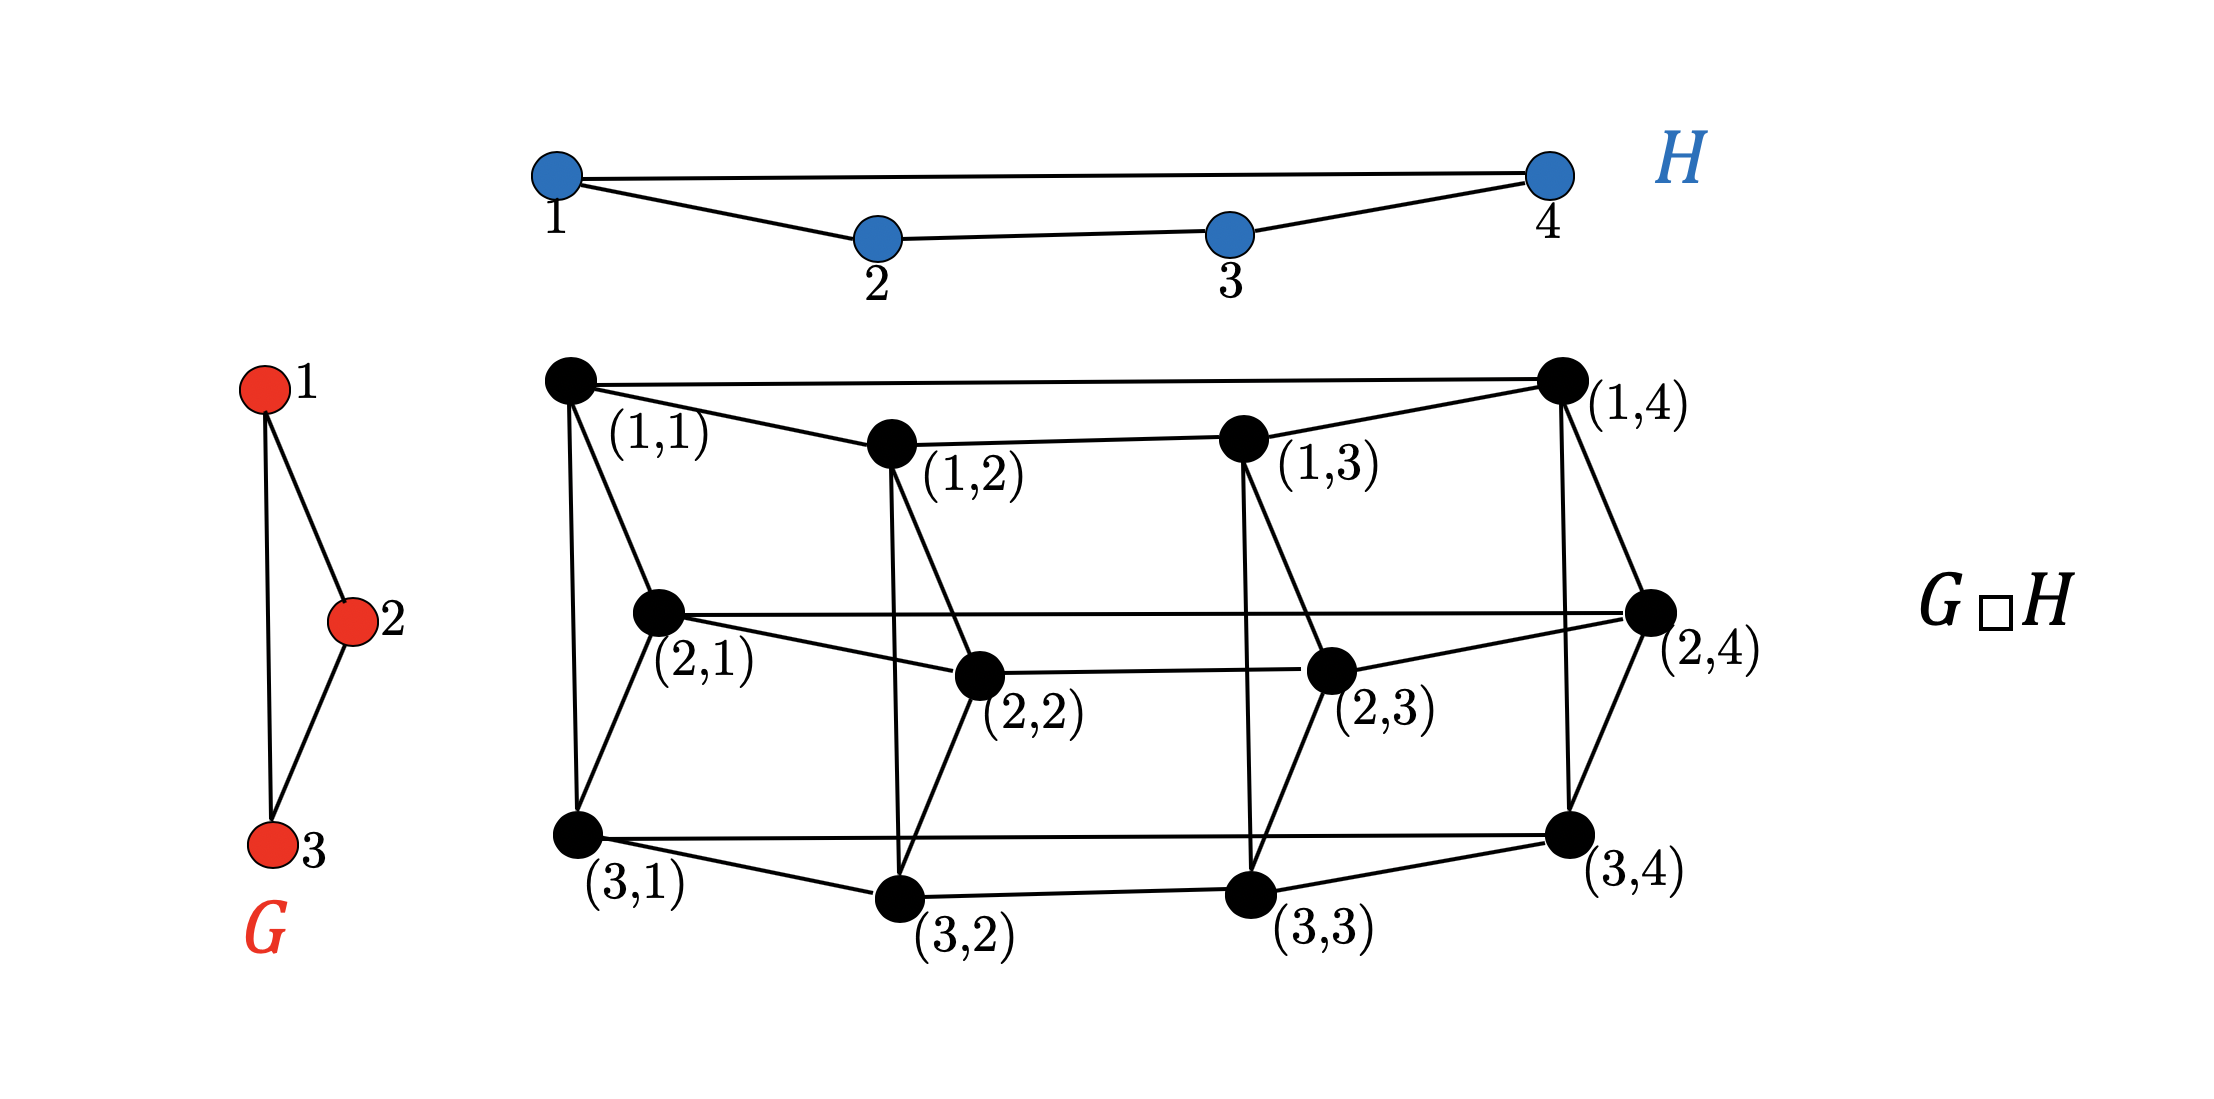
\includegraphics[width=0.9\linewidth]{fig/CpWest.png}
	\caption{$C_3 \square C_4$ an example of the Cartesian product}
	\label{fig:p2}
\end{figure}

Our contributions can be summarized as follows:

1) In \cite{Fitz16}, Fitzpatrick et al. conjectured that $\zn(G \square H) \leq \zn(G) + \zn(H)$. In \ref{conj-proof} We prove this conjecture and
use it to show that $\zn(Q_n) = \ceil*{\frac{2n}{3}}$. 

2) In \ref{capturetime}, we provide a new bound on {\it capture time} of {\it zombies and survivor} game played on the Cartesian
product of two graphs. 

3) We introduce a variation of {\it zombies and survivor} game, in which the zombie player is restricted to winning in a
limited number of moves in \ref{np-capturetime}, and prove it belongs to {\it NP-Hard} class of problems.


4) In \ref{np-zombienumber}, we prove that the original {\it zombies and survivor} game belongs to {\it NP-Hard} class
of problems.


\section{Zombie number of the Cartesian product of two graphs}\label{conj-proof}

To prove $\zn(G \square H) \leq \zn(G) + \zn(H)$, we show that $\zn(G) + \zn(H)$ zombies are enough for the zombie player to
capture the survivor on $G \square H$.

To explain the proof we first need to define some notations. Assume $H$ and $G$ have $m$ and $n$ vertices,
respectively. 

We define $G_{i}$ as the induced subgraph by all vertices $(u,v)$ in $G \square H$, where $v=i$. Similarly $H_{j}$ is
defined as the induced subgraph by vertices $(u,v)$ in $G \square H$, where $u=j$.

In the Cartesian product of $G$ and $H$, each $G_{i}$ $(1 \leq i \leq m)$ is isomorphic to $G$, and each $H_{j}$ $(1
\leq j \leq n)$ is isomorphic to $H$. We name the common vertex between $G_{i}$ and $H_{j}$, $(j,i)$. Also $(x,y)$ is
the vertex where the survivor is located. Figure \ref{fig:p1} illustrates these definitions.

A {\it G-edge} is an edge in one of the $G_{i}$s and an {\it H-edge} is an edge in one of the $H_{j}$s. A {\it G-move}
is a move made on a {\it G-edge}. Similarly, an {\it H-Move} is a move made on an {\it H-edge}. If the survivor decides
to remain in its current vertex, this move is considered both a {\it G-move} and an {\it H-move}. 

$dist_I(j,k)$ is the distance between $j$ and $k$ vertices on a graph $I$. Length of a path $P$ is shown by $len(P)$. 

For vertex $(u,v)$, $G$-equivalent vertex, is vertex $u$ on graph $G$, and $H$-equivalent vertex, is vertex $v$ on graph
$H$. $G$-equivalent graph is a graph where we put each zombie and the survivor on its $G$-equivalent vertex.
$H$-equivalent graph is defined in the same way.


\begin{figure}[h!]
	
	\centering
	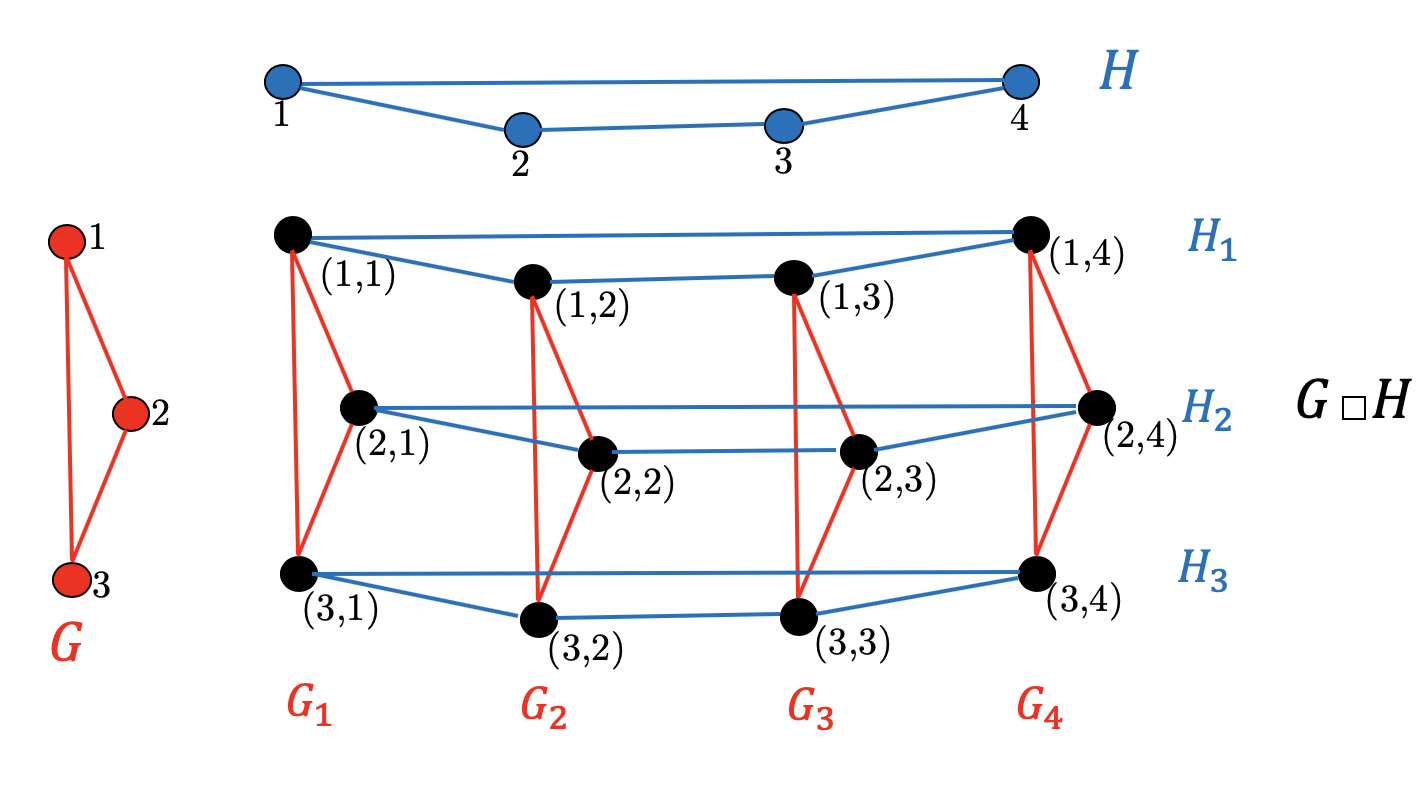
\includegraphics[width=0.9\textwidth]{fig/cp3.png}
	%\includegraphics[width=200pt]{cp.png}
	\caption{$G \square H$, $G_i$s, and $H_i$s.}
	\label{fig:p1}
\end{figure}



\begin{lemma} \label{shortestpathlemma}
	$dist_{G \square H}((x,y),(u,v)) = dist_G(x,u) + dist_H(y,v)$.
\end{lemma}
\begin{proof}
	Since there is a path from $(x,y)$ to $(x,v)$ with length $dist_H(y,v)$ and a path from $(x,v)$ to $(u,v)$ of length
	$dist_G(x,u)$, we only need to prove there can be no path with length less than $dist_G(x,u) + dist_H(y,v)$.
	Suppose not, this path uses some {\it G-move}s and some {\it H-move}s. If a {\it G-move} is followed by an {\it
	H-move} (or vice-versa), then we can swap these moves and still end up in the same vertex. For example if $(u_1,v_1)
	\rightarrow (u_2,v_1) \rightarrow (u_2,v_2)$ is happening, we can do $(u_1,v_1) \rightarrow (u_1,v_2) \rightarrow
	(u_2,v_2)$. Since we can swap each two moves of different type, suppose all {\it G-move}s happen before all {\it
	H-move}s in the shortest path. Since this path has a length less than $dist_G(x,u) + dist_H(y,v)$, we have found a
	path in either $G$ between $x$ and $u$, with length less than $dist_G(x,u)$, or in $H$ between $y$ and $v$, with
	length less than $dist_H(y,v)$, which is a contradiction. Thus the statement holds.
\end{proof}




\begin{theorem}
	\label{T2}
	$\zn(G \square H) \leq \zn(G) + \zn(H)$.
\end{theorem}

\begin{proof}
	We provide a winning strategy for the Cartesian product of $G$ and $H$ using $\zn(G)+\zn(H)$ zombies. First, we place
	$\zn(G)$ zombies, that have a winning strategy on a single $G$, $G_{a = 1}$ and call them {\it G-zombie}s. We do the
	same for $H_{b = 1}$ and call them {\it H-zombie}s.


	Consider one of the shortest paths between vertices $a$ (the index of $G$-subgraph shared by {\it G-zombie}s) and
	$y$ in $H$ and call it $p_H$. We also define $p_G$ in the same manner between $b$ and $x$.


	On each zombie turn, if $a \neq y$, each {\it G-zombie} will move along the $p_H$ path in its corresponding $H$
	subgraph. According to Lemma \ref{shortestpathlemma}, since zombies' and survivor's equivalents on $H$ are getting
	closer, thus their actual vertices on $G \square H$ are getting closer as well and this move is possible. Since they
	are all moving along similar paths (in their corresponding $H$-subgraphs) they will still share the same
	$G$-subgraph. Now consider when $a = y$, {\it G-zombie}s will play their winning strategy (that they had on a single
	$G$) in this case. This move is also possible since in $G$'s strategy, zombies would get closer to survivor on each
	turn. If $a = y$ and survivor makes an {\it H-move}, {\it G-zombie}s will maintain their positioning by mimicking
	the exact same move on their corresponding $H$. This means for those turns that $a=y$ holds, if we consider the
	$G$-equivalent graph between {\it G-zombie}s and the survivor, it is just like a simple game played on a single $G$.
	{\it H-zombie}s will follow the same strategy but in their corresponding environment.
	
	
	Suppose using this strategy $G \square H$ is {\it survivor-win}, then the survivor must either do infinite {\it
	G-move}s or infinite {\it H-move}s. Without loss of generality, suppose the survivor makes infinite {\it H-move}s,
	we prove that this is not possible. After $len(p_G)$ number of {\it H-move}s, {\it H-zombie}s will get to $H_x$. Now
	for each {\it G-move} made by survivor and having zombies chasing him, nothing changes in their $H$-equivalent
	graph. Since the survivor can do infinite {\it H-move}s and prevent being caught, it means that the survivor could
	also avoid being caught on a single $H$ which contradicts our assumption.
	
\end{proof}
An example for further understanding can be found at \ref{CartesianProductExample}.

\begin{corollary}
	\label{C3}
	$\zn(Q_{n}) \leq \ceil*{\frac{2n}{3}}$
\end{corollary}
\begin{proof}
	We prove this by using both induction and the theorem proved above. First note that the Cartesian product of
	hypercube graphs $Q_{m}$ and $Q_{n}$ is equal to $Q_{m+n}$. It is easy to see $\zn(Q_3) = 2$, $\zn(Q_2) = 2$, and
	$\zn(Q_1) = 1$. For $n > 3$, we consider $Q_n$ as the Cartesian product of $Q_3$ and $Q_{n-3}$. Using the induction
	base, we know that $\zn(Q_{n-3}) \leq \ceil*{\frac{2n - 6}{3}}$. According to the proved conjecture $\zn(Q_n) \leq
	\zn(Q_{n-3}) + \zn(Q_3)$ and $\zn(Q_{n-3}) \leq \ceil*{\frac{2n - 6}{3}} = \ceil*{\frac{2n}{3}} - 2$, we can see that
	$\zn(Q_n) \leq \ceil*{\frac{2n}{3}}$.
\end{proof}

It is already proved that at least $\ceil*{\frac{2n}{3}}$ zombies are needed to capture one survivor on graph $Q_n$
(Theorem 16 of \cite{Fitz16}):

\begin{theorem}
	\label{T4}
	For each integer $n \geq 1$, $\zn(Q_n) \geq \ceil*{\frac{2n}{3}} $.
\end{theorem}

Combining {\it Corollary \ref{C3}} and {\it Theorem \ref{T4}} we can conclude that $\zn(Q_n) = \ceil*{\frac{2n}{3}}$.
This proves Conjecture 18 from \cite{Fitz16} which is already proved in \cite{Offner19} with a different method. 
	

\section{Capture time in Cartesian product of graphs}\label{capturetime}
	We define a new parameter, {\it capture time} of the game, noted as $capt(G,z_c)$, which represents the maximum
	number of moves that survivor can avoid being caught on a graph $G$, when the zombie player uses $z_c$ zombies. Zombie
	player tries to make $capt(G,z_c)$ as least as possible, while survivor tries to maximize it. Also $diam(G)$ is the
	length of $G$'s diameter.

	\begin{theorem}
		\label{T5}
		$capt( G \square H, z_G + z_H ) \leq diam(G) + diam(H) + capt(G, z_G) + capt(H, z_H)$
	\end{theorem}
	\begin{proof}
		By using $z_G$ zombies as {\it G-zombie}s and $z_H$ zombies as {\it H-zombie}s, and having them follow the same
		set of moves provided in theorem \ref{T2}, we show that survivor's {\it G-move}s cannot exceed $diam(H)
		+ capt(G, z_G)$. With the same conclusion, it can be shown that {\it H-move}s cannot exceed $diam(G) + capt(H, z_H)$
		as well.

		According to the definition of the diameter of a graph, after at most first $diam(H)$ {\it G-move}s that
		survivor makes, $a = y$ holds. Now since for each {\it G-move} made from now on by survivor, {\it G-zombie}s can
		follow their strategy on a $G$ graph, and after at most $capt(G,z_G)$ {\it G-move}s, survivor will be captured. 
		
		Since each of survivor's moves is either a {\it G-move} or an {\it H-move} or both, total number of moves cannot
		exceed $diam(G) + diam(H) + capt(G, z_G) + capt(H, z_H)$.
	\end{proof}
\section{Limited capture time zombie number problem is NP-Hard}\label{np-capturetime}

	{\it NP-hardness} (non-deterministic polynomial-time hardness) is, in computational complexity theory, a class of
	problems that are informally "at least as hard as the hardest problems in NP class". A problem is assigned to the NP
	(non-deterministic polynomial time) class if it is solvable in polynomial time by a non-deterministic Turing
	machine.

	A well known example of an NP-hard problem is the {\it dominating-set} problem in graph theory. A {\it
	dominating-set} for a graph $G$ is a subset $D$ of $V(G)$ such that every vertex not in $D$ is adjacent to at least
	one member of $D$. The domination number $\gamma(G)$ is the number of vertices in the smallest dominating-set for
	$G$.

	We define $Lc\zn(G,k)$ ({\it limited capture time zombie number}) as the minimum number of zombies needed so that
	zombie player is able to capture the survivor in at most $k$ moves on graph $G$. 

	Also $N_G[u]$ represents the set of neighbors of $u$ in graph $G$.
	
	$LC\NPZ_k$ problem is defined as below:
	{\newline}
	INSTANCE: Let $G = (V,E)$ be a simple undirected graph. Given a graph $G$ and two positive integers $z_c$ and $k$.
	{\newline}
	QUESTION: Is $Lc\zn(G,k) \leq z_c$ ? In other words, can the zombie player capture the survivor after at most $k$ moves using 
	$z_c$ zombies in graph $G$ ?
	{\newline}
	{\newline}
	The dominating-set problem is defined below:
	{\newline}
	INSTANCE: Let $G = (V,E)$ be a simple undirected graph. Given a graph $G$ and a positive integer $d$.
	{\newline}
	QUESTION: Is $\gamma(G) \leq d$ ?

	\begin{theorem}
		$LC\NPZ_k$ $\in$ NP-Hard
	\end{theorem}
	\begin{proof}
		We prove this by reducing the dominating-set problem to $LC\NPZ_k$ in polynomial time.

		To have a better understanding, consider the case where $k=1$. For zombie player being able to capture the
		survivor in one move, every vertex not occupied by a zombie, should have a zombie neighbor. This is exactly the
		definition of a dominating-set. This simply shows that $LC\NPZ_1 \in$ NP-Hard class.

		Now consider $k$ to be an arbitrary integer bigger than 1. We construct a new graph $G'_k$ from $G$. Suppose $G$
		has $n$ vertices. For each vertex $v \in V(G)$, we add a {\it new} path with $k$ vertices ending in $v$ (as
		shown in figure \ref{fig:p7}), and name each {\it new} vertex $(v,i)$ for $1 \leq i < k$. 

		\begin{figure}[h!]
			\centering
			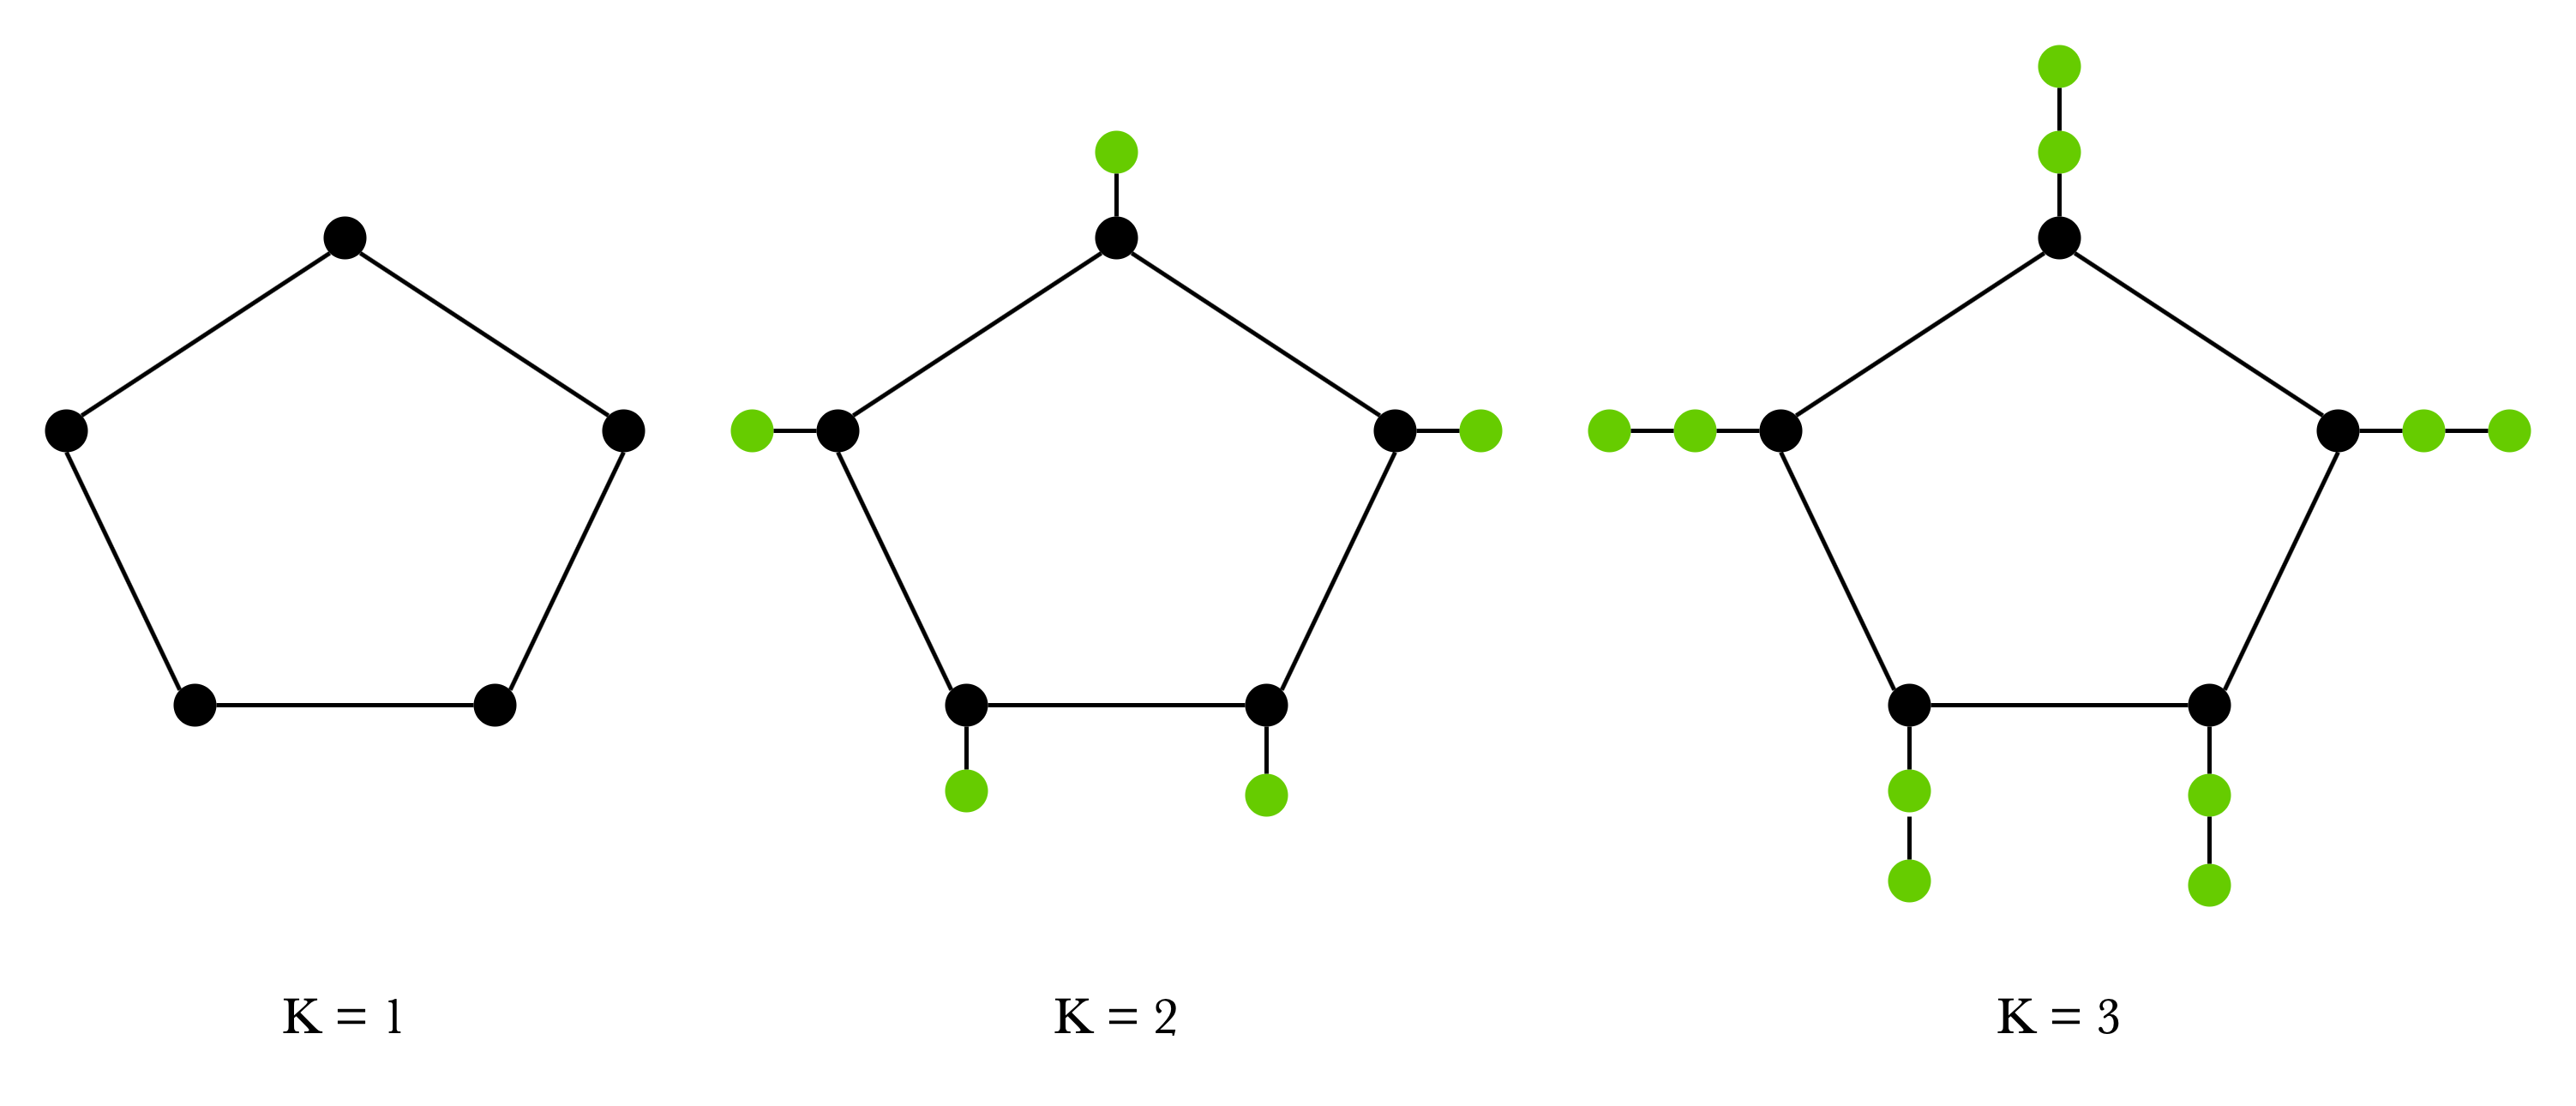
\includegraphics[width=0.9\linewidth]{fig/LCZ.png}
			\caption{$G'_k$ obtained from $G = C_5$ where for $k = 1,2,3$}
			\label{fig:p7}
		\end{figure}		


		$|V(G'_k)| = nk$ is of $O(n)$. Thus creating $G'_k$ can be done in polynomial time. Consider set $S'$ as zombies'
		initial vertices on $G'_k$, so that zombies are able to capture the survivor within $k$ moves. For each vertex $v \in
		S'$ or $(v,i) \in S'$ add $v$ to a new set of $G$'s vertices, $S$. If there is a vertex $u \in G$ not dominated by
		$S$, then there is no vertex $v$ such that $v \in S'$ and $v \in N_{G'_k}[u] \cup \{u, (u,1 \leq i < k)\}$. By having
		the survivor in vertex $(u, k-1)$, there is no vertex at distance $k$ or less from him, which means he will not
		be captured. Thus $\gamma(G) \leq Lc\zn(G'_k,k)$ holds.
		
		Now for each vertex $v$ in one of $G$'s smallest dominating-sets, place a zombie on vertex $v$ of $G'_k$. These
		zombies can capture the survivor in at most $k$ moves. To show this, consider survivor's initial vertex, if it
		is not a {\it new}ly added vertex, he can be captured in one move. Now suppose survivor is initially on $(u,i)$. Since
		$u$ is dominated by a zombie, after zombies' first move, survivor will be trapped inside the $u$'s path, and would
		be captured in at most $k$ moves. Therefore, $Lc\zn(G'_k,k) \leq \gamma(G)$.

		By combining these results, $Lc\zn(G'_k,k) = \gamma(G)$. Therefore the dominating-set problem is reduced to
		$LC\NPZ_k$.

	\end{proof}

	\begin{lemma}
		\label{limit-moves}
		Let $n$ be the number of vertices of graph $G$. If survivor can avoid being captured on $G$ after $(n + 1)
		\times n \times diam(G)$ moves, he can forever avoid being captured on $G$.
	\end{lemma}
	\begin{proof}
		Define $zombieDist$ as the sum of the distances between each zombie and the survivor. It is not hard to see that
		after each two rounds of play, that is each player has played once, $zombieDist$ will not increase, since
		zombies are always getting closer to the survivor. Now we show that if $zombieDist$ does not strictly decrease
		after each player takes turn for $n + 1$ times, survivor can avoid being captured forever. Consider the sequence
		of vertices occupied by survivor in $n + 1$ consecutive moves. By pigeonhole principle, one vertex has been seen
		by survivor at least twice. If survivor keeps repeating those moves, he will maintain his distance from zombies
		and will avoid being captured forever.

		Therefore, for a graph $G$ which zombie-player can win, after each $(n + 1)$ moves, $zombieDist$ should strictly
		decrease. $zombieDist$ is at most $n \times diam(G)$, since there is not more than $n$ zombies and each zombie is at distance
		at most $diam(G)$ from survivor (this bound can be easily improved). Thus, after $(n + 1) \times n \times diam(G)$ moves, zombies would
		capture the survivor.
	\end{proof}

	By using this lemma, we can see $LC\NPZ_k$ problem for $k > (n + 1) \times n \times diam(G)$ and a graph with $n$ vertices are the same as
	the problem $LC\NPZ_{(n + 1) \times n \times diam(G)}$, and by solving $LC\NPZ_{(n + 1) \times n \times diam(G)}$ for $G$, we get $\zn(G)$ as well.


	
	\section{Zombie Number Problem is NP-Hard}\label{np-zombienumber}

	Now define zombie number ($\NPZ$) problem:
	{\newline}
	INSTANCE: Let $G = (V,E)$ be a simple undirected graph. Given graph $G$ and an integer $z_c$.
	{\newline}
	QUESTION: Is $\zn (G) \leq z_c$?

	\begin{theorem}
		$\NPZ \in$ NP-Hard class.
	\end{theorem}
	\begin{proof}
		We reduce dominating-set problem to $\NPZ$.

		To do this, we add $n$ new complete bipartite graphs, $K_{n,n}$, to $G$. We call the newly obtained graph $H$,
		and call the $G$-subgraph simply as $G$, and the $i$-th $(1 \leq i \leq n)$ bipartite subgraph as $K_i$.
		$(i,j,b)$ represents the $j$-th vertex in $K_i$'s part $b$ ($b = 1,2$) . For each vertex $(i,j,b)$ we connect it
		to vertices $j$ and $N_G[j]$ (See figure \ref{fig:p8}). Since we are adding $2n^2$ new vertices, building $H$
		can be done in polynomial time.

		\begin{figure}[h!]
			\centering
			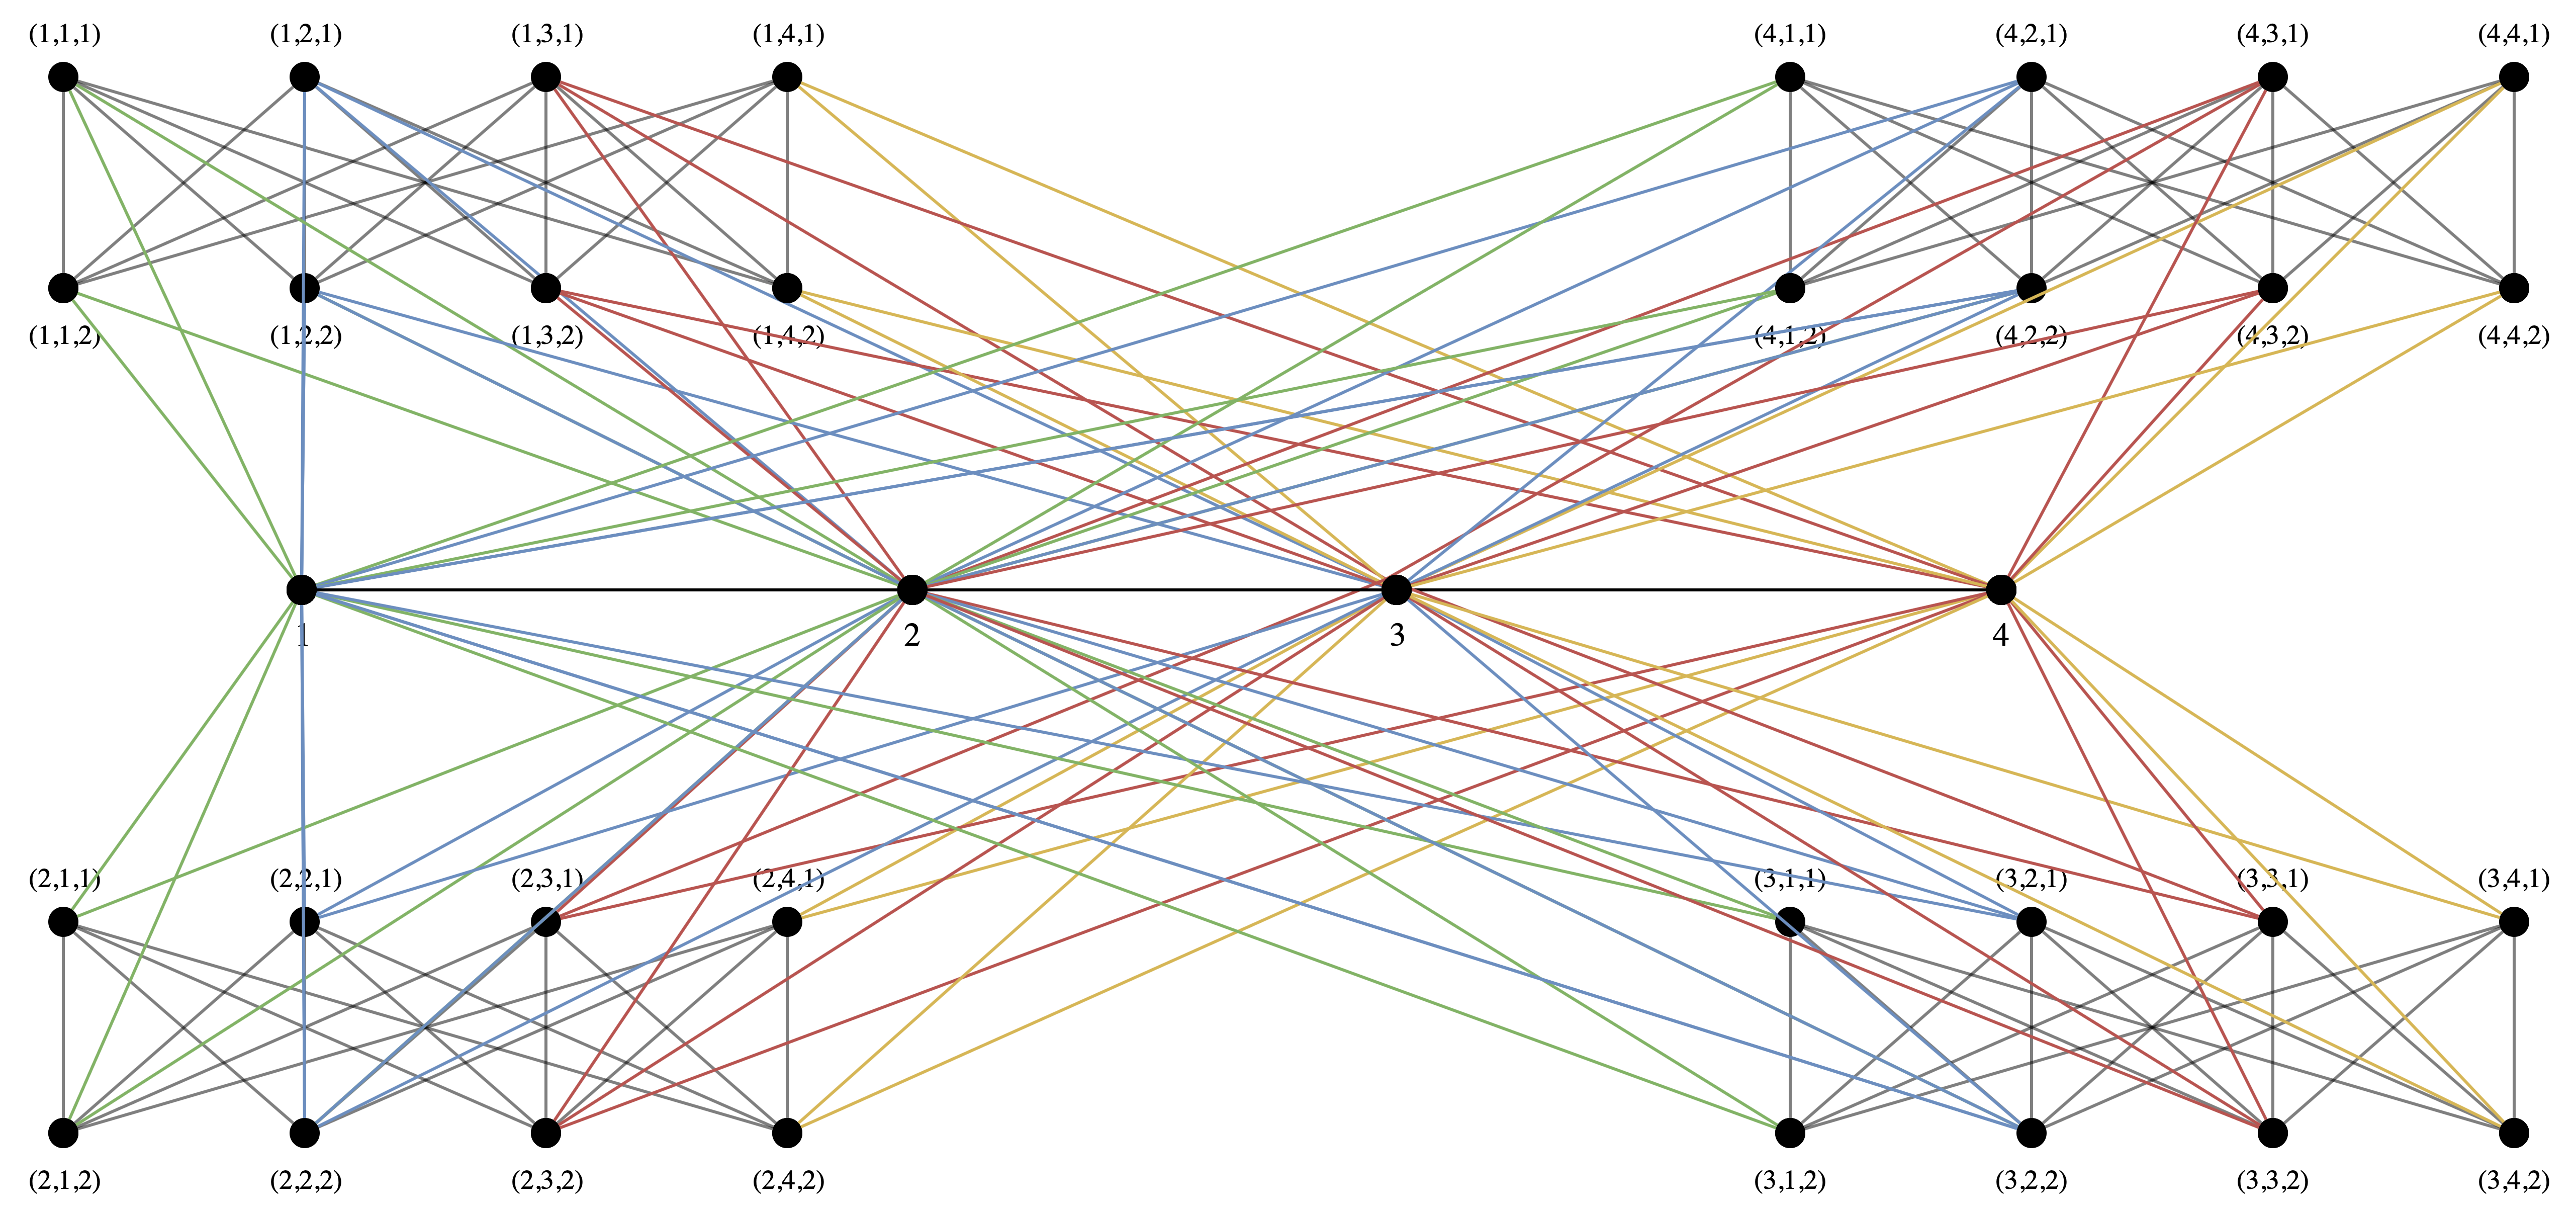
\includegraphics[width=0.9\linewidth]{fig/sec5.png}
			\caption{$H$ obtained from $P_4$, zombie player needs at least $\gamma(P_4) = 2$ zombies to win}
			\label{fig:p8}
		\end{figure}

		By having zombies on each vertex of $G$'s dominating-set, survivor will be captured on the first move and zombie
		player wins. Thus, $\zn(H) \leq \gamma(G)$. Now suppose we have zombies less than the domination number of
		graph: $z_c < \gamma(G)$. We prove survivor can avoid being captured.

		Suppose zombie player has placed his zombies. Since we have $n$ bipartite subgraphs and $z_c < n$, there is a
		bipartite subgraph, without any zombies in it ($k$-th bipartite graph). Since the vertices corresponding to
		these zombies are not dominating $G$, there is a vertex $v$, not dominated by them. We place the survivor on
		vertex $(k,v,b = 1)$ and therefore, survivor has no neighbors occupied by a zombie. On each survivor turn, there
		is a vertex $v$ in $G$ not dominated by a zombie, therefore survivor will move to vertex $(k,v,3 - b)$. We prove
		by following this move, he will survive. On zombies' turn, zombie player has zombies on either $G$ or some $K_i$
		$(i \neq k)$ or $K_k$. Initially there is no zombie in $K_k$, this means whenever a zombie wants to join $K_k$,
		it has to be in $G$ in order to reach $K_k$, as there is no connection between $K_i$-subgraphs. Zombies in $G$
		(e.g. at vertex $u$) are at distance 2 from survivor $(u \rightarrow (k,u,3 - b) \rightarrow (k,v,b))$, which
		means after their move all of them should be at one of $(k,v,b)$'s neighbors, that is, $v , N_G[v] $ or, $ (k,1
		\leq i \leq n,3 - b)$. Therefore, each zombie joining $K_k$ does not share the same partition as survivor's.
		Survivor now moves to $(k,v,3-b)$ and will be sharing the same partition as zombies' in $K_k$. As survivor does
		not have any neighbors in $G$ or $K_k$ on each zombie player's turn, he will not be captured. Therefore,
		$\gamma(G) \leq \zn(H)$.

		It is now proved that $\zn(H) = \gamma(G)$, thus the dominating-set problem is reduced to $\NPZ$.

	\end{proof}
\begin{thebibliography}{999}
	
	\bibitem{Fitz16}
	Fitzpatrick, Shannon L., J. Howell, Margaret-Ellen Messinger, and David A. Pike. "A deterministic version of the
	game of zombies and survivors on graphs." Discrete Applied Mathematics 213 (2016): 1-12.
	\bibitem{Offner19}
	Offner, David, and Kerry Ojakian. "Comparing the power of cops to zombies in pursuit-evasion games." Discrete
	Applied Mathematics (2019).
	\bibitem{West02}
	West, Douglas B. "Introduction to Graph Theory." Prentice hall, (1996).
\end{thebibliography}

\newpage
\appendix
\section{An example for zombie number of Cartesian product of two graphs} \label{CartesianProductExample}
\begin{example} $\zn(P_3 \square P_4 ) = 2$
\end{example}

\begin{figure}[h!]
	\centering
	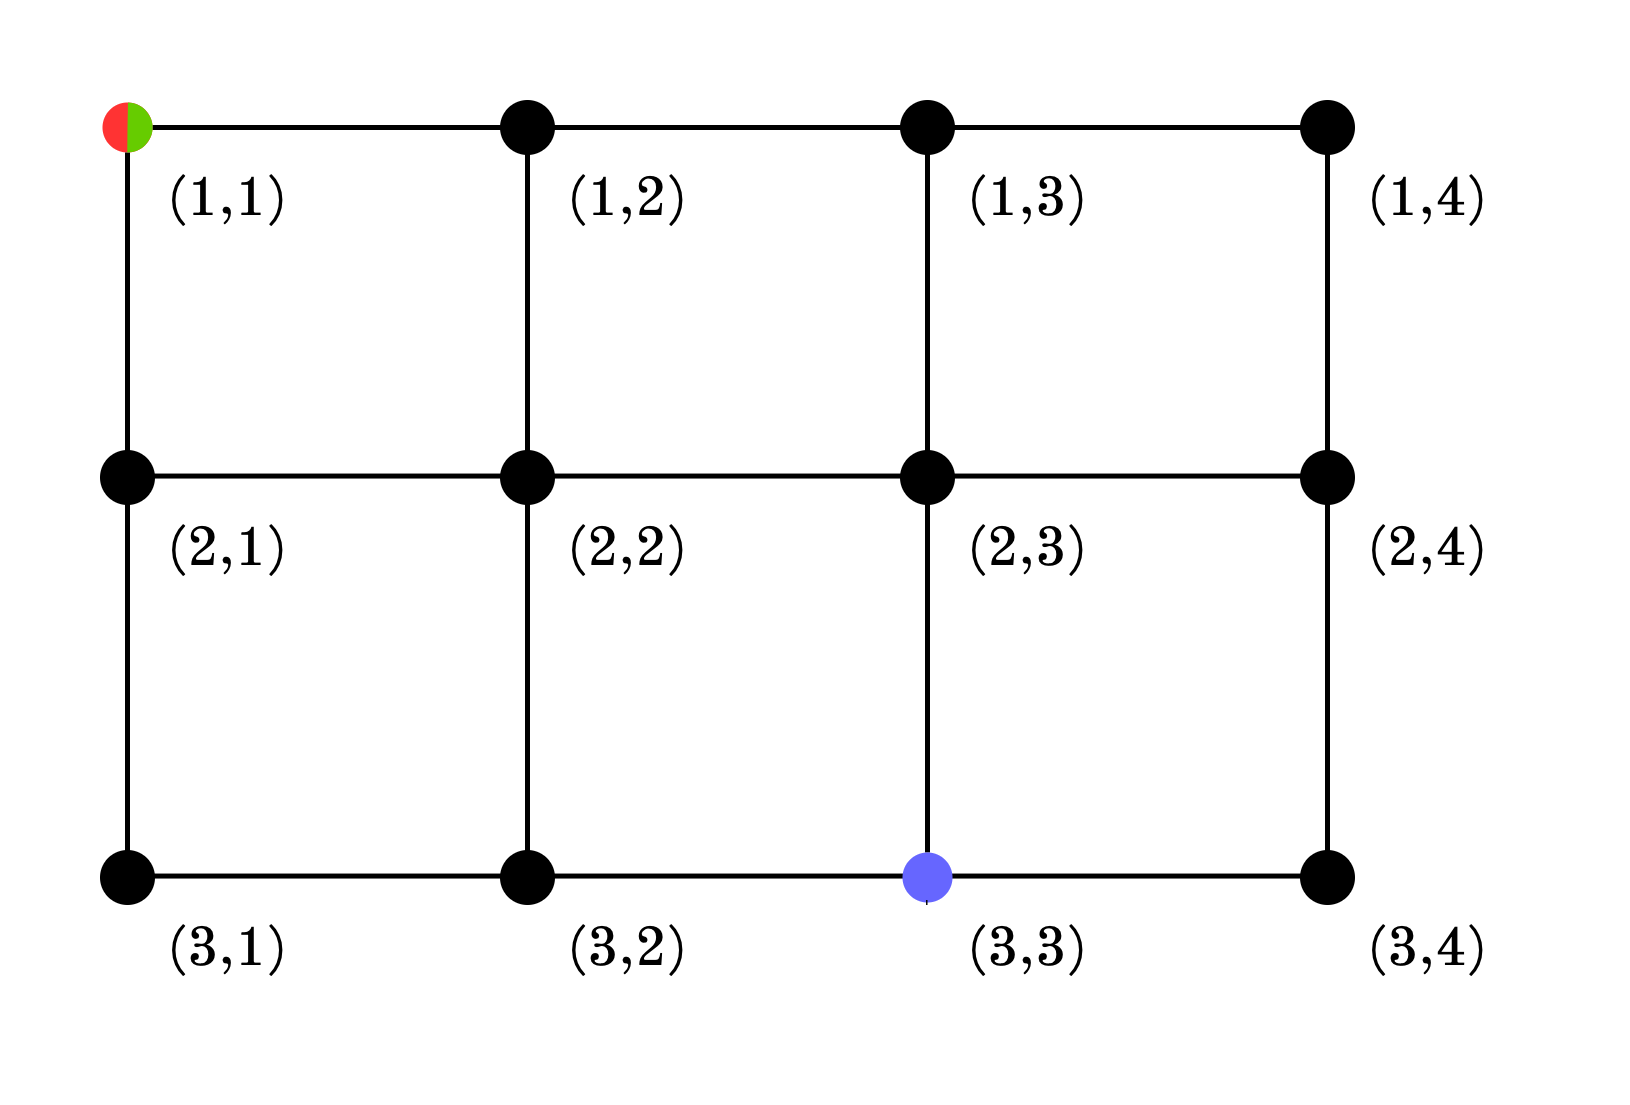
\includegraphics[width=0.5\linewidth]{fig/p34m1.png}
	\caption{$P_3 \square P_4$ and initial vertices}
	\label{fig:p3}
\end{figure}

It is easy to show that $\zn(P_3) = \zn(P_4) = 1$. On each of these path graphs, zombie's initial position could be any
vertex of the graph. For this example, we put the {\it G-zombie} and {\it H-zombie} ($G = P_3$ and $H = P_4$) both on
vertex $(1,1)$. We show the survivor with blue color, {\it H-zombie} with red, and {\it G-zombie} with green. {\it
G-zombie} will try to get to the same $G_{i}$ as survivor's which is $G_3$ using an {\it H-edge}. {\it H-zombie} will
try to get to $H_3$ (See figure \ref{fig:p4}).

\begin{figure}[h!]
	\centering
	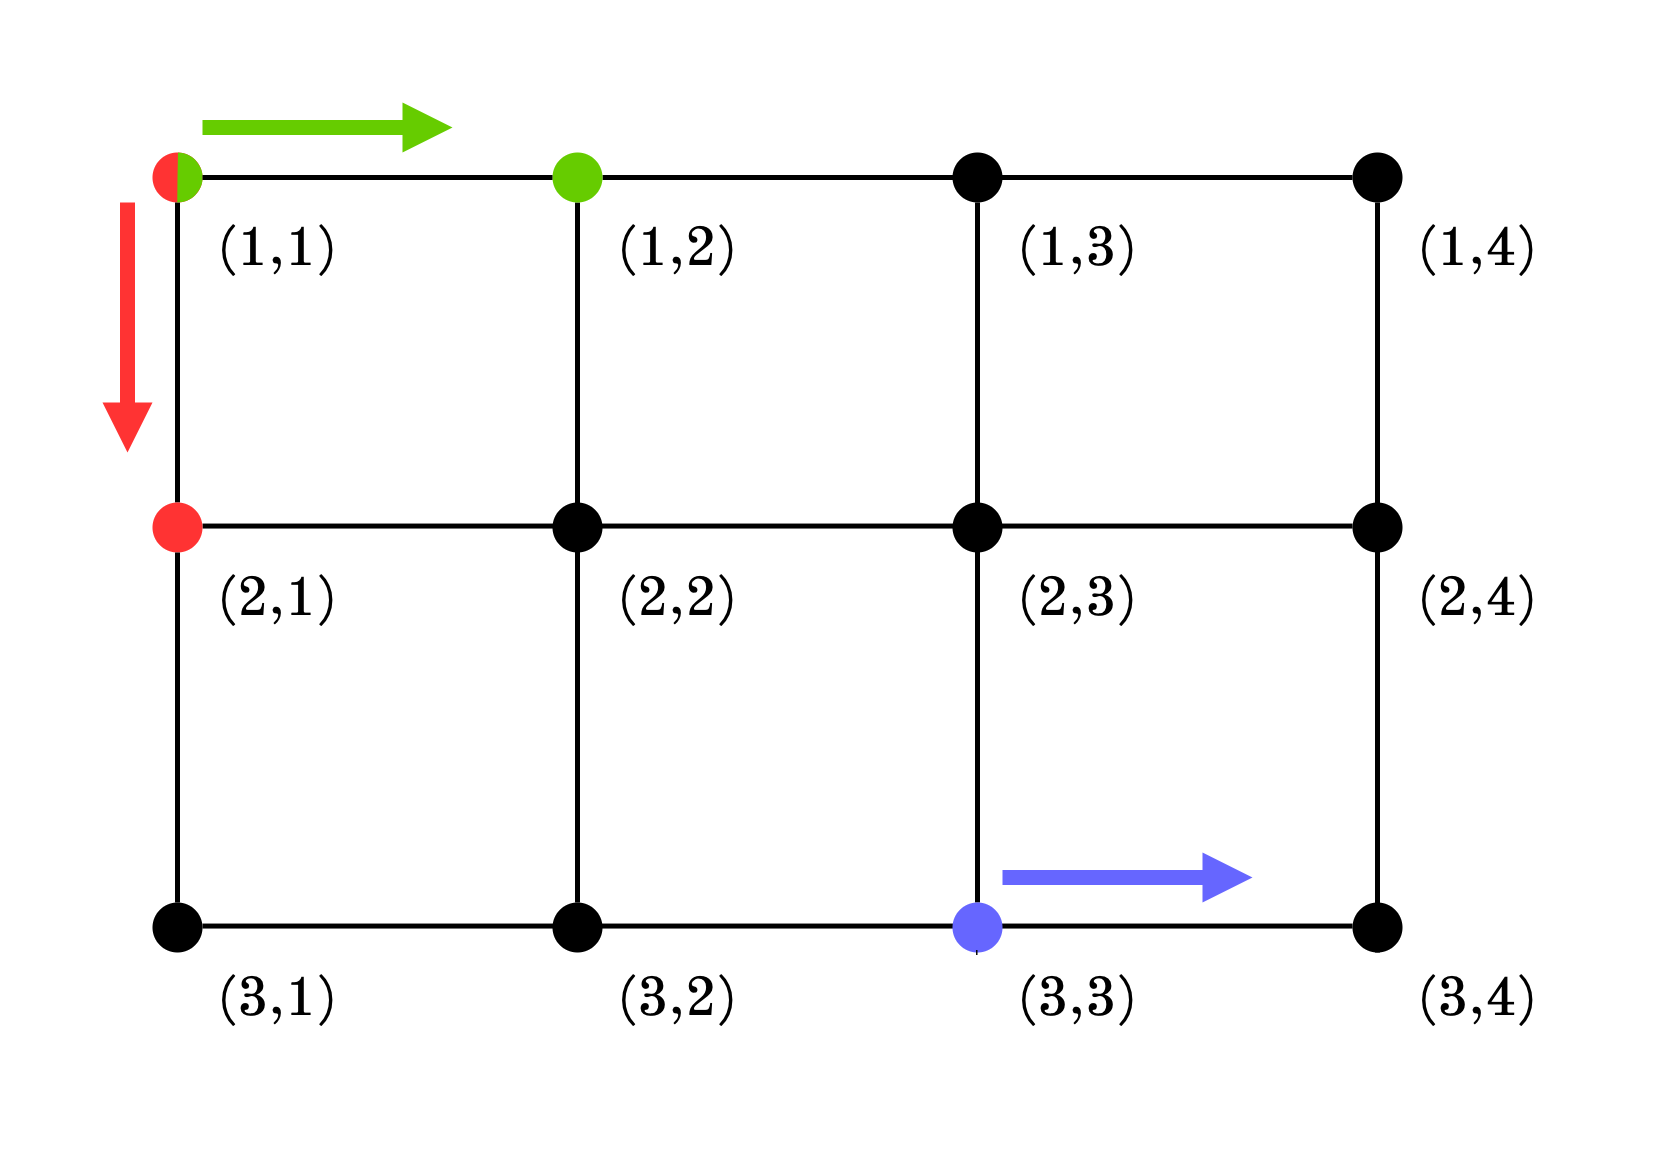
\includegraphics[width=0.5\linewidth]{fig/p34m2.png}
	\caption{First move of players}
	\label{fig:p4}
\end{figure}

After zombies' move the survivor must move. No matter what move he makes, either {\it G-zombie} has made itself closer
to $H_x$ or {\it H-zombie} has made itself closer to $G_y$. In this case, {\it H-zombie} got closer to $H_x$. Since
neither {\it H or G-zombie}s share $H_x$ or $G_y$ with the survivor, they will still try to achieve that (See figure \ref{fig:p5}).

\begin{figure}[h!]
	\centering
	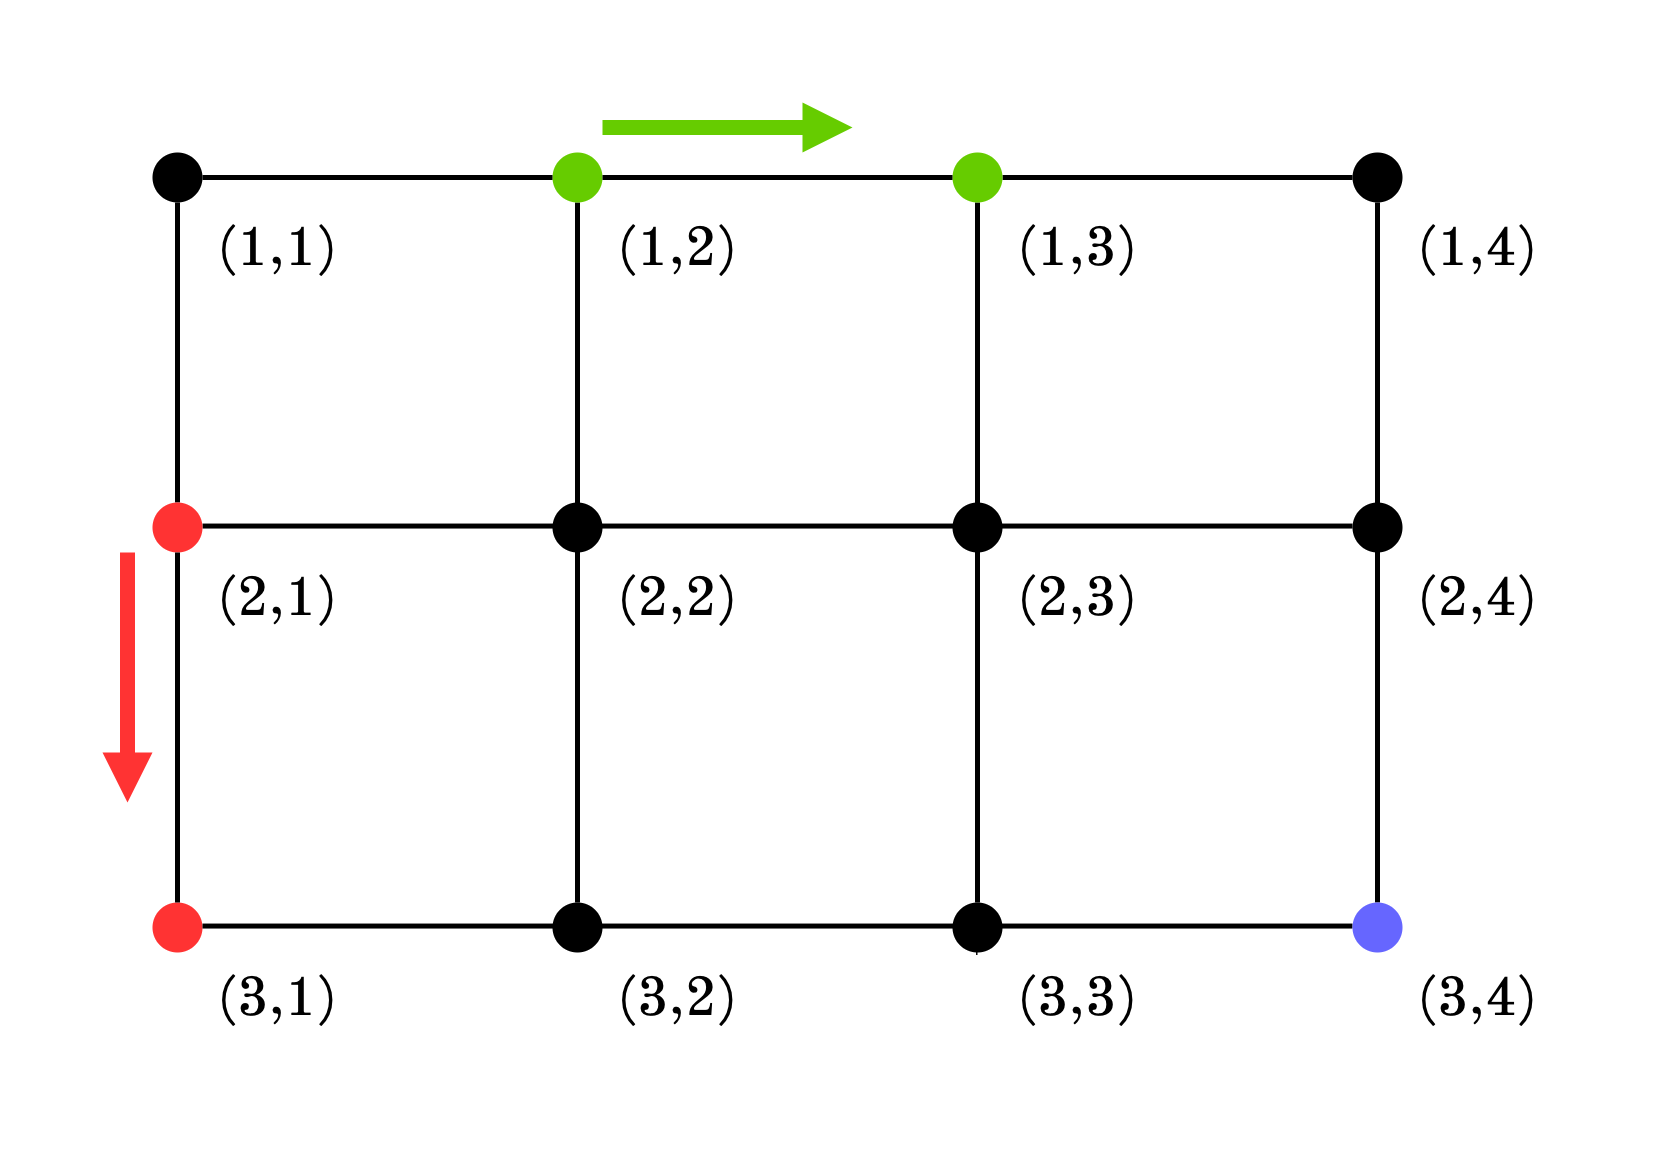
\includegraphics[width=0.5\linewidth]{fig/p34m3.png}
	\caption{Second move made by zombies, third in total}
	\label{fig:p5}
\end{figure}

Now {\it H-zombie} shares the same copy of $H$ as survivor and it is survivor's turn. If survivor moves to another
$H_i$, {\it H-zombie} will mimic the move. If survivor makes an {\it H-move}, {\it H-zombie} will do whatever it did on
a single $H$ for capturing the survivor. This means survivor cannot do infinite {\it H-move}s. Thus for him being able
to survive he has to do infinite {\it G-move}s, which again leads to {\it G-zombie} capturing him. For other moves, you
can see figure \ref{fig:p6}.

\begin{figure}[h!]
	\centering
	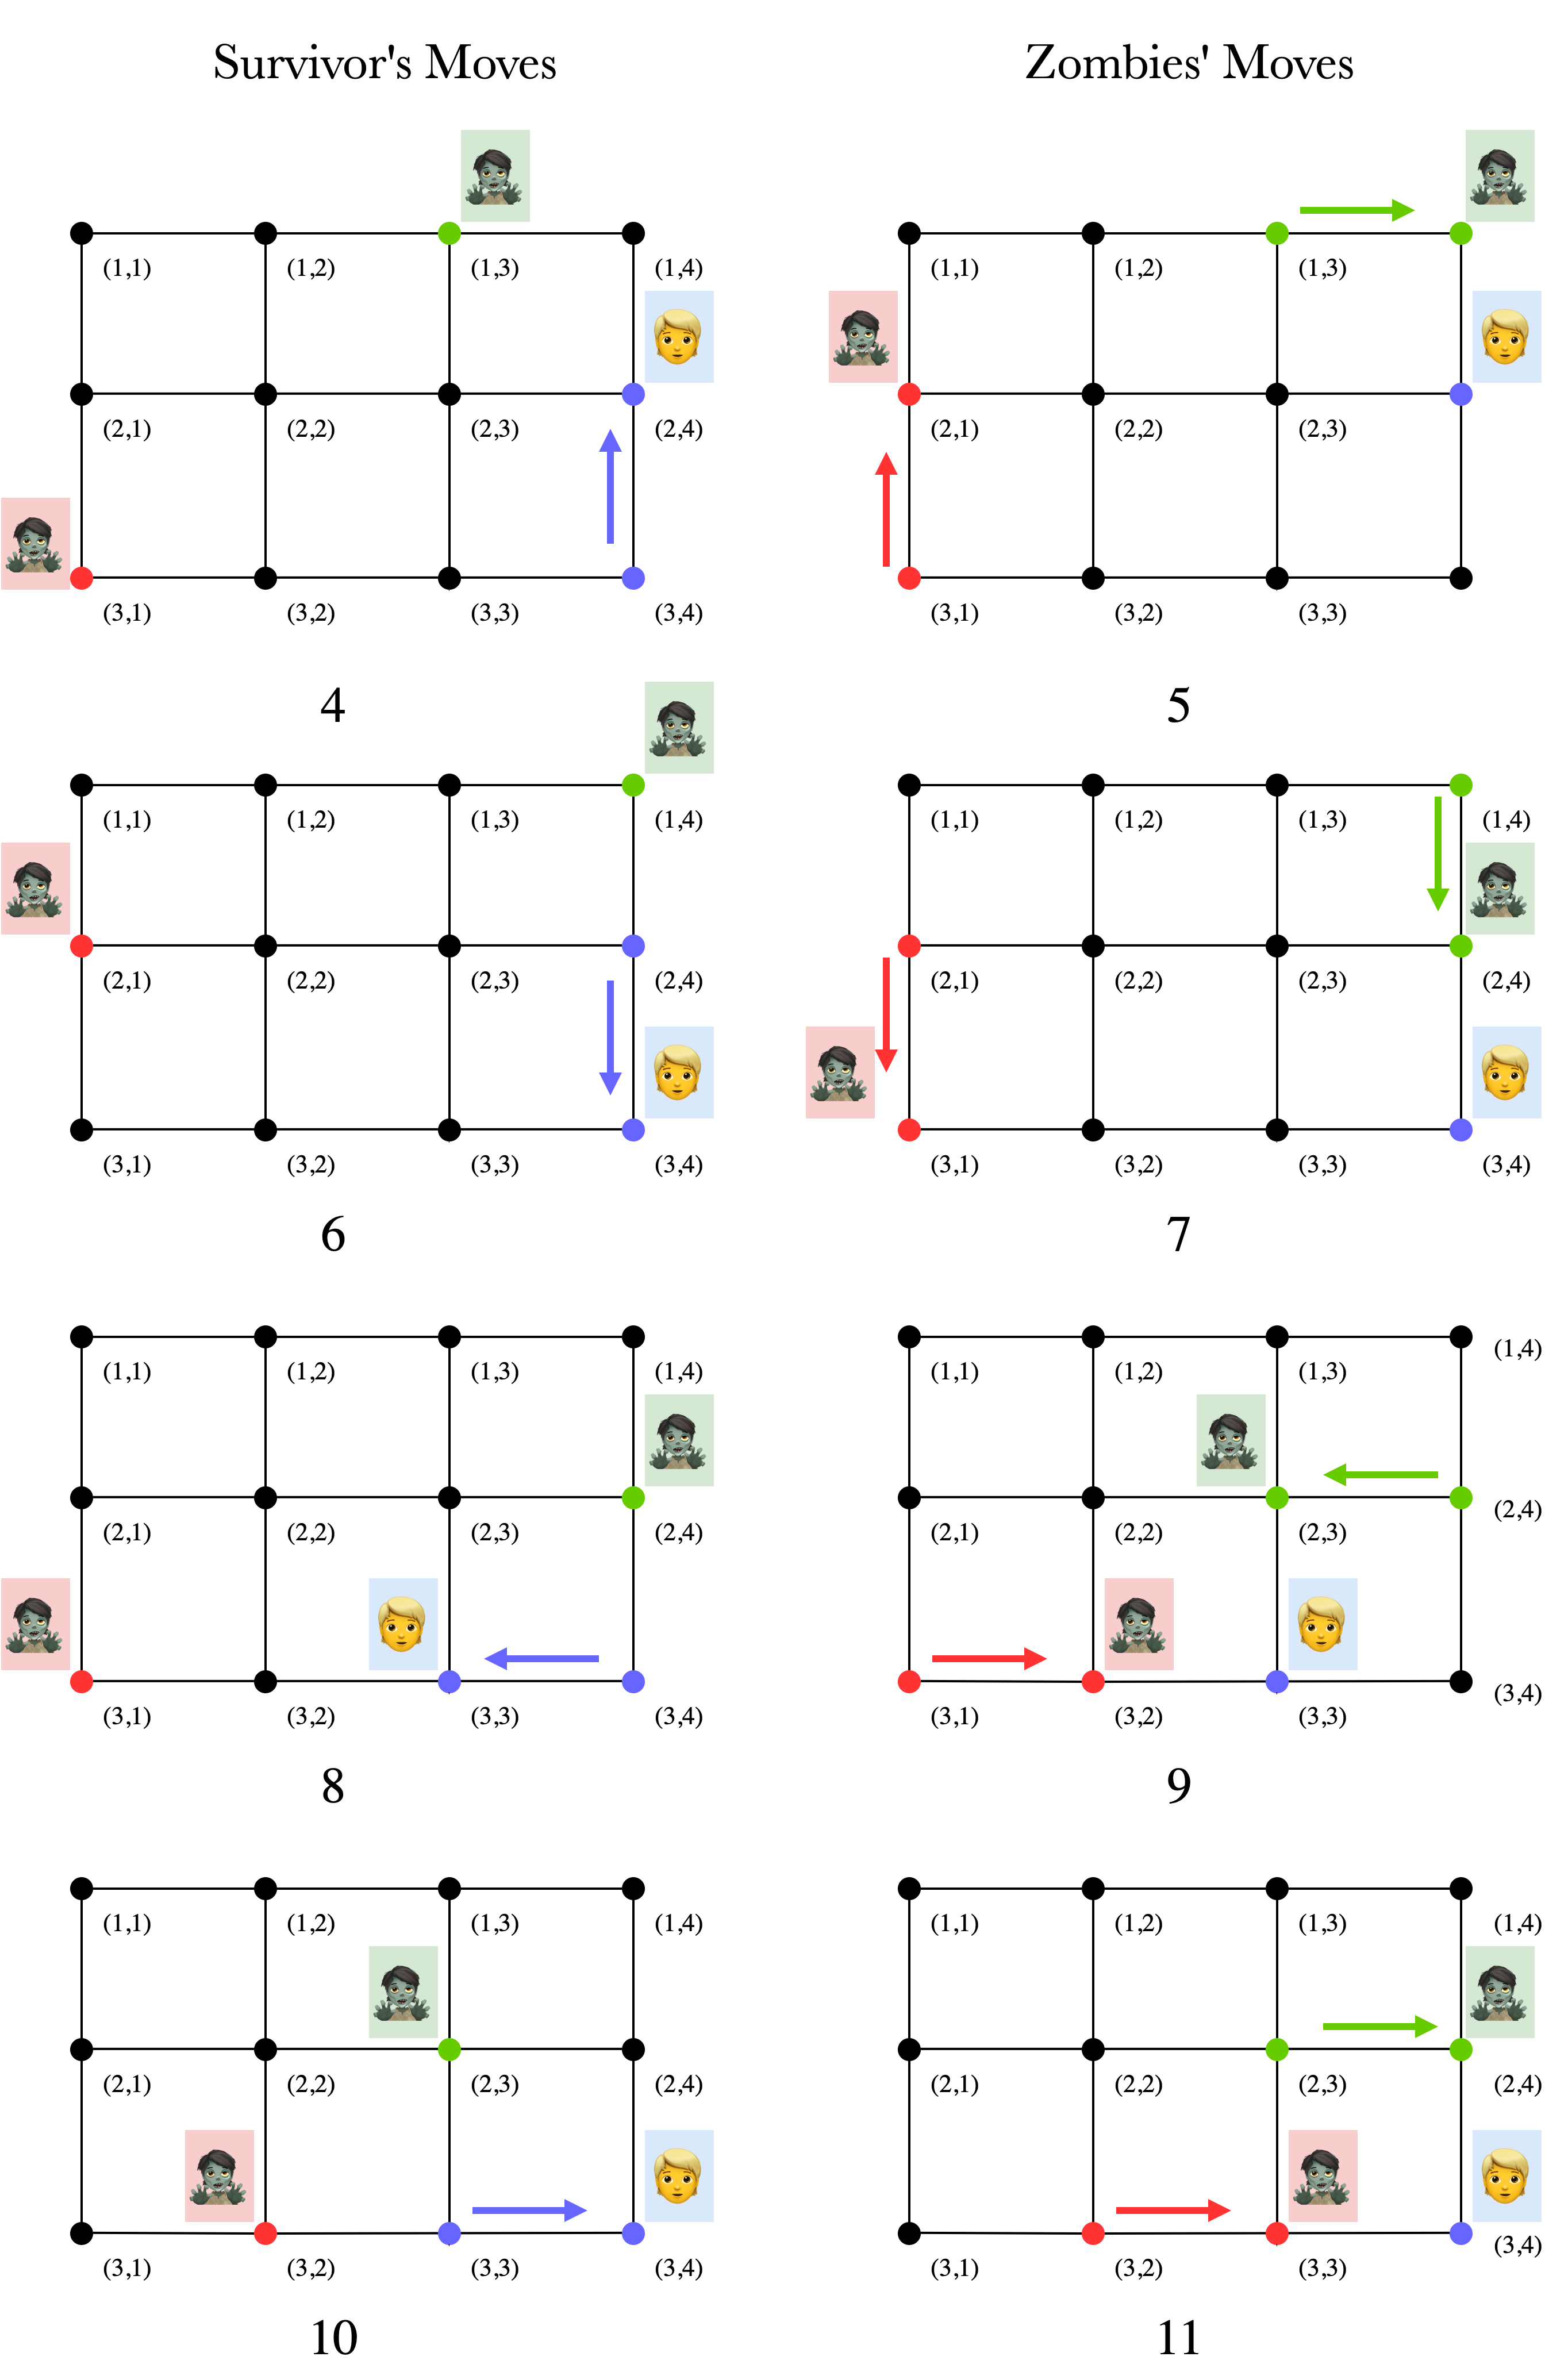
\includegraphics[width=1\linewidth]{fig/p34m6.png}
	\caption{Other moves made by players}
	\label{fig:p6}
\end{figure}

	
\end{document}